\section{Augmented Cube}
In this section, we calculated the full camera matrix in each frame and we used that for projecting a 3D cube into that frame. After that we tried to do the texture mapping on the faces of the cube we projected.

We tried two methods for calculating the projection camera. First method uses chessboard obtained from an arbitrary "first" image, and computes the homography between the first frame and the currently processed frame. It then uses the homography to construct the projection matrix for the camera. The second method uses just the chessboard pattern in the current frame to establish the world origin and relate the camera position towards it.

The second method gives us a better result, because the first method computes the homography between two frames and because the frames can have relative distortion with each other and an absolute distortion it will slightly worse result.

Now that we found the camera matrix with both methods for testing them we tried to project the chesspattern points in the world coordinate system to the current camera view. All points were projected to the right place in the image so we moved to the next step.

In this step we drew the world coordinate axes attached to the chesspattern plane and then we projected the cube into the current view again attached to the pattern plane. In order to do this, we had a representation of the cube in object coordinates, and we have positioned it in the world without any translation, rotation or scaling. Thanks to this, it was possible for us to treat the coordinates of the cube object coordinate system as if they were in the world coordinate system. Otherwise we would have to transform them from object coordinate system into world coordinate system.

 \begin{figure}[h!]
	\centering
	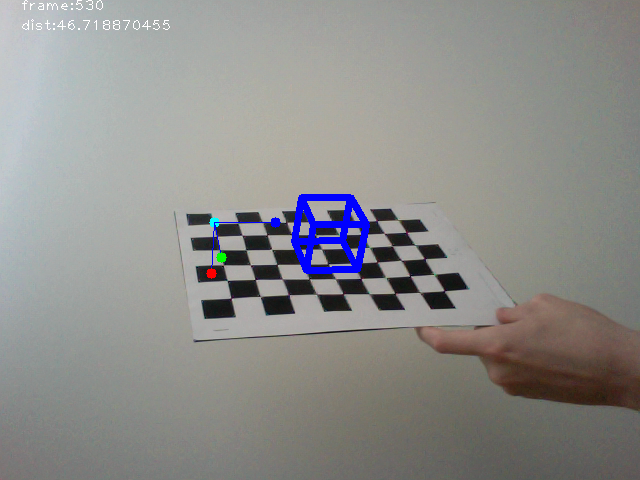
\includegraphics[width=\textwidth]{Handin3/images/wireframe.png}
	\caption{Wireframe Cube}
	\label{fig:wireframe}
\end{figure}

To draw a wireframe model in Figure \ref{fig:wireframe} we simply take a pair of points from the cube that form an edge, project them using the projection matrix we calculated before to obtain their positions in the 2D image and then just draw a line between them.
